\documentclass[runningheads]{llncs}

\usepackage[T1]{fontenc}

\usepackage{adjustbox}
\usepackage{algorithmic}
\usepackage{amsmath,amssymb,amsfonts}
\usepackage{array}
\usepackage{cite}
\usepackage{colortbl}
\usepackage{diagbox}
\usepackage{gensymb}
\usepackage{graphicx}
\usepackage{makecell}
\usepackage{multirow}
\usepackage{textcomp}
\usepackage{tikz}
\usepackage{xcolor}
\usepackage{subcaption}
\captionsetup{compatibility=false}


\newcommand*\circled[1]{\tikz[baseline=(char.base)]{
		\node[shape=circle, draw, inner sep=0pt, minimum size=1em, font=\scriptsize] (char) {#1};
}}

\definecolor{commentgray}{RGB}{110,110,110}

\newcommand{\rcmtinline}[1]{\hfill\textcolor{commentgray}{\footnotesize /* #1 */}}
\newcommand{\rcmtbelow}[1]{\hfill\textcolor{commentgray}{\footnotesize /* #1 */}}
\graphicspath{{figure/}}

\begin{document}


% An Environment-aware and Safety-constrained Hybrid Rule Conflicts Detection Framework in Smart Homes
% Environment-aware Hybrid Detection of Safety-constrained Rule Conflicts in Smart Home
% Hybrid Detection of Rule Conflicts in Smart Home
\title{Environment-aware Hybrid Detection of Safety-constrained Rule Conflicts in Smart Home}
% \titlerunning{Environment-aware Hybrid Detection of Safety-constrained Rule Conflicts in Smart Home}
\titlerunning{Hybrid Detection of Rule Conflicts in Smart Home}

\author{Yaodong Zhang$^1$, Jian Mao$^{1,2}$, Qixiao Lin$^1$, Qiange Liu$^1$, and Yan Huo$^3$}
\authorrunning{Y. Zhang et al.}

\institute{$^1$Beihang University, Beijing 100083, China\\
$^2$Tianmushan Laboratory, Hangzhou 311121, China\\
$^3$Beijing Jiaotong University, Beijing 100044, China\\
}

\maketitle

\begin{abstract}

% Smart home platforms rely on automation rules to coordinate devices and sensors, but independently configured automation rules can interact through shared entities and zone-dependent physical-channel propagation, leading to unintended and unsafe behaviors. Existing rule conflict detectors often over-approximate potential interactions without considering zone-specific propagation and user-specific safety preferences. Moreover, they rarely confirm whether a suspected conflict is actually activated at runtime, leading to false positives. We present a hybrid framework that combines offline static analysis with runtime dynamic monitoring for rule conflict detection. The framework incorporates zone-dependent physical-channel propagation and a user-defined Entity Safety Configuration to focus on safety-relevant candidate rule conflicts, and uses runtime assertion verification to confirm activated conflicts under the current system state. Implemented on Home Assistant and evaluated in a multi-zone testbed with 17 automation rules, our framework detects all manually confirmed conflict cases and eliminates nine false positives reported by IoTMediator, while keeping runtime verification overhead at the millisecond level.

Smart home platforms utilize automation rules to coordinate devices and sensors. These rules often interact through shared devices and physical channels, such as temperature or illumination, leading to unintended behaviors. Existing rule conflict detection approaches often identify logical overlaps between automation rules without determining whether the underlying interaction is physically relevant in the current deployment or harmful under the target application scenario. As a result, they may over-report benign interactions as rule conflicts, especially when physical propagation is constrained by zone boundaries or when user-specific safety requirements differ across scenarios. In this paper, we propose a hybrid framework that combines offline static analysis with runtime dynamic monitoring. The framework utilizes a Trigger-Condition-Action-Environment (TCAE) model to account for zone-dependent physical interactions. We introduce an entity safety configuration that allows users to define safety boundaries, transforming potential interactions into a Rule Conflict Dependency Graph (RCDG). A runtime monitor then performs assertion verification to confirm whether suspected conflicts are actually triggered under the current system state. We implemented the framework on Home Assistant and evaluated it in a multi-zone environment. The results show that our approach identifies all confirmed conflicts and eliminates nine false positives reported by the state-of-the-art tool IoTMediator. The runtime verification maintains a millisecond-level overhead, ensuring system efficiency.

\keywords{Smart home · rule conflict · hybrid detection · runtime verification}

\end{abstract}

\section{Introduction}

The smart home is an important application domain of the Internet of Things (IoT), where automation rules connect devices, sensors, and environmental events to automate daily tasks. Most automation rules follow the Trigger-Condition-Action (TCA) model. As the number of automation rules grows, unintended rule interaction becomes more likely and may further evolve into rule conflicts, disrupting expected automation and causing security or safety risks \cite{huang2023survey,trimananda2020understanding,chi2023detecting}. For example, enabling a sprinkler upon smoke detection may indirectly trigger a leak-response rule that closes the water valve, undermining firefighting \cite{chi2023detecting}.

Recent work has further investigated rule conflict detection in IoT-based smart homes \cite{huang2023survey,huang2021conflict,li2020diac,trimananda2020understanding,yagita2015application,chaki2020fine,yu2022tapinspector,pradeep2021automating}. Existing approaches mainly include security-policy-based methods and pattern-based methods. Security-policy-based methods check whether rule execution violates predefined safety or security policies, often by modeling automation rules and checking safety properties over the resulting models \cite{celik2018soteria,celik2019iotguard,ding2021iotsafe,hsu2019safechain,sun2014conflict,ibrhim2020formal}. Pattern-based methods identify suspicious interaction structures, such as race condition, chained triggering, and conflicting actions \cite{alhanahnah2022iotcom,chi2020cross,chi2023detecting,li2020diac,xiao2019a3id,trimananda2020understanding,chaki2020fine}. Although these approaches are useful, they still have difficulty determining whether a rule interaction should be treated as a candidate rule conflict in a specific smart home setting.

This challenge arises from three factors. First, rule conflict is context-dependent. Because smart homes are heterogeneous and user preferences differ, the same rule interaction may be benign in one deployment but unsafe in another, leading to false positives or false negatives under generic detection logic. Second, many interactions propagate through physical channels with zone-dependent propagation (e.g., thermal isolation), so detectors that ignore zone boundaries may infer non-existent interactions \cite{celik2019iotguard,alhanahnah2022iotcom,chen2019multi,wang2019charting}. Third, runtime confirmation of candidate rule conflicts remains difficult. Although static analysis is comprehensive, it often over-approximates without the current system state. Existing dynamic or hybrid systems can monitor rule events and physical contexts \cite{ding2021iotsafe}, yet they do not explicitly verify whether a candidate conflict edge is actually activated at rule-trigger time.

To address these limitations, we draw three insights. Rule interaction exists not only at the logical layer but also propagates through physical channels in different zones, which requires a rule model that captures both spatial and environmental effects. Rule interaction and rule conflict should be explicitly distinguished, and the user-defined Entity Safety Configuration is used to determine whether a rule interaction should be retained as a candidate rule conflict. Finally, combining candidate conflict edges derived from static analysis with the current system state through assertion verification can reduce the over-approximation introduced by static analysis alone. Based on these observations, we propose a hybrid framework that combines offline static analysis with runtime dynamic monitoring. In the static phase, we apply formal verification to construct the Rule Interaction Dependency Graph (RIDG) and then extract the Rule Conflict Dependency Graph (RCDG) according to the user-defined Entity Safety Configuration. In the runtime phase, we use assertion verification to check whether candidate conflict edges in the RCDG are activated under the current system state, thereby identifying impending rule conflicts at runtime.

In summary, our main contributions are as follows:

\begin{itemize}
	\item We extend automation rule modeling to the Trigger-Condition-Action-Environment (TCAE) model and use the RIDG, the RCDG, and the Entity Safety Configuration to distinguish general rule interaction from candidate rule conflicts.

	\item We design a hybrid detection framework in which static analysis pre-screens interactions and limits runtime checking to candidate conflict edges instead of the full rule set.

	\item We implement a runtime mechanism based on assertion verification that combines the current system state with temporal evidence to determine whether a candidate conflict edge is activated; in our testbed, it eliminates nine false positives reported by IoTMediator while keeping runtime overhead at the millisecond level.
\end{itemize}
\section{Motivating Example and Problem Analysis}

\begin{figure}[htbp]
	\centering
	
\includegraphics[width=0.9\textwidth]{figure/motivated_example.png}
	\caption{Motivating Example}
	\label{motivated_example}
\end{figure}

% We use a motivating example to show why rule logic alone is insufficient to determine whether a rule interaction should be retained as a candidate rule conflict. Figure~\ref{motivated_example} shows two zones in a smart home: the bedroom on the left and the greenhouse on the right. The bedroom contains a heater (\circled{1}) and a window (\circled{2}); the greenhouse contains a heater (\circled{3}) and a skylight (\circled{4}). Consider two automation rules configured in the greenhouse: R1 turns on the heater at sunset, and R2 opens the skylight and turns off the heater when the temperature reaches 30\celsius.

% This example reveals three observations. \textbf{User preferences influence whether a rule interaction should be treated as benign or as a candidate rule conflict.} In the greenhouse, the interaction between R1 and R2 can be an expected feedback loop for temperature control. With the same rule logic in the bedroom, however, opening the window at night may create an intrusion risk. In practice, such preferences enter the detection process through the Entity Safety Configuration. \textbf{Physical propagation depends on zone and environmental characteristics.} A heater in one zone does not necessarily affect the temperature in another isolated zone, so a detector that assumes heating always raises temperature may report false positives by inferring non-existent interactions. \textbf{Harmfulness requires explicit safety baselines.} Even when an interaction edge exists, the system still needs preferred safe states to determine whether the result should be treated as a candidate rule conflict. For example, opening the greenhouse skylight may be acceptable, whereas opening the bedroom window may violate the preferred safe states defined in the Entity Safety Configuration.

% These observations motivate our design, which utilizes Physical Channel Configuration to model spatial effects and Entity Safety Configuration to encode user preferences. These inputs enable the system to filter rule interactions into candidate conflicts during static analysis and verify them via dynamic monitoring.

We illustrate the challenges of rule conflict detection through a representative smart home scenario involving two distinct zones. Figure~\ref{motivated_example} depicts a bedroom containing a heater and a window , alongside a greenhouse equipped with a heater and a skylight window. Automation rules are configured to manage the indoor temperature in both areas. For instance, a rule might activate the heater at sunset to maintain warmth. A separate rule triggers the opening of the window or skylight if the temperature exceeds 30\celsius. Although the underlying logic of these rules remains identical across both zones, the resulting physical interactions lead to fundamentally different safety outcomes. Opening the skylight in the greenhouse serves as a benign ventilation mechanism to maintain an optimal growth environment. The identical rule execution in the bedroom creates a security vulnerability by providing a potential entry point for intruders at night.

This scenario highlights several limitations in existing conflict detection approaches. Current tools often assume that any device influencing a common physical channel, such as temperature, constitutes a potential interaction. This assumption ignores the reality that \textbf{physical propagation is highly dependent on spatial boundaries}. A heater operating in the bedroom does not influence the environmental state of the isolated greenhouse. Systems lacking this spatial awareness frequently report non-existent interactions, leading to a high volume of false positives. Furthermore, \textbf{the definition of a rule conflict is related to the specific application scenario and user intent}. As Figure~\ref{motivated_example} demonstrated, the same automation logic can manifest as either a benign environmental adjustment or a severe security vulnerability depending on the context. Purely logic-based detectors fail to distinguish between these cases because they lack the safety baselines required to evaluate the harmfulness of an interaction.

Our approach addresses these issues by decoupling rule interactions from safety violations. We recognize that \textbf{an interaction only qualifies as a conflict if it satisfies both physical reachability and a violation of user-defined safety requirements}. This insight motivates a two-stage analysis detection framework guided by specific environmental and safety configurations. The framework utilizes a physical channel configuration to model the propagation characteristics within each zone. This ensures that only physically possible interactions are mapped into the Rule Interaction Dependency Graph (RIDG). To refine this graph, we incorporate an entity safety configuration that encodes the preferred safe states for each zone. This allows the system to prune benign interactions and focus exclusively on candidates that threaten the security of the environment, which are represented in the Rule Conflict Dependency Graph (RCDG). Finally, the system employs runtime assertion verification to bridge the gap between static modeling and actual execution. By monitoring real-time device states, the framework confirms whether these candidate conflicts are actually triggered, thereby eliminating false alarms stemming from static over-approximation.
\section{Design}

\subsection{Overview}
\begin{figure*}[t]
	\centering
	
\includegraphics[width=0.7\textwidth]{figure/overall_design.png}
	\caption{Overall Architecture of Our Approach}
	\label{overall_design}
\end{figure*}

We propose a hybrid framework that combines offline static analysis with runtime dynamic monitoring for rule conflict detection in the smart home. As shown in Figure~\ref{overall_design}, the framework consists of two phases. In the static phase, the system parses automation configurations together with the Physical Channel Configuration to build enhanced rule models, applies formal verification to construct the RIDG, and then uses the Entity Safety Configuration to prune the RIDG and extract the RCDG, which retains the interaction edges corresponding to candidate rule conflicts. In the runtime phase, the system monitors rule events, checks whether triggered rules correspond to nodes in the RCDG, and uses assertion verification with the current system state to determine whether a candidate conflict edge is activated. If so, the candidate rule conflict associated with that edge is reported as an impending rule conflict. In essence, the static phase first determines whether a rule interaction is physically relevant in the current deployment and then checks whether it violates the safety boundary of the target application scenario; the runtime phase confirms whether such a candidate conflict is actually activated.

\subsection{Static Analysis}

We begin by clarifying how automation rules interact. The action of one rule may affect the trigger, condition, or action of another rule either directly or through physical channels. We therefore consider six types of rule interaction: Trigger Interaction, Condition Interaction, Action Interaction, Indirect Trigger Interaction, Indirect Condition Interaction, and Indirect Action Interaction. These categories provide the basis for constructing the RIDG, after which the Entity Safety Configuration is applied to the identified interaction edges to retain candidate rule conflicts.

Automation rules are usually represented by Trigger (T), Condition (C), and Action (A). However, the TCA model alone cannot represent indirect interaction through physical channels. We therefore extend it to the TCAE model by introducing environmental attributes $E_T$, $E_C$, and $E_A$, where each element is written as $e=(zone, channel, trend)$. Here, $zone$ denotes the affected zone, $channel$ denotes the physical quantity, and $trend$ denotes whether the quantity increases or decreases. For example, if a rule turns on a bedroom heater, its action may include $\langle bedroom, temperature, increase \rangle$ in $E_A$. A rule is thus modeled as $R=\langle T, C, A, E_T, E_C, E_A \rangle$, which allows the system to represent indirect interaction and zone boundaries. The Physical Channel Configuration is used to determine these environmental attributes from the deployment setting.

After modeling automation rules with TCAE, we use formal verification to identify pairwise rule interaction and organize the results as a directed graph. We define the RIDG as $G_I=(V,E_I)$, where each vertex in $V$ denotes an automation rule and each directed edge in $E_I$ denotes that one rule may affect another through a direct or indirect interaction. For each pair of rules $R_i$ and $R_j$, the verifier checks whether they satisfy any formal condition in Table~\ref{Formal_Analysis_Expression}. If so, a directed edge $R_i \rightarrow R_j$ is added to the RIDG. The RIDG therefore captures the general rule interactions that are logically or physically possible under the current rule set and deployment setting.

Table~\ref{Formal_Analysis_Expression} summarizes the formal verification rules. Assume $R_1$ and $R_2$ are configured in the same system. The symbol $\rightarrow$ denotes that an action or environmental effect facilitates a trigger or condition, whereas $\nrightarrow$ denotes that it prevents a condition from being satisfied. For physical-channel attributes, $\bot$ denotes that two attributes have the same $zone$ and $channel$ but opposite $trend$, or that two actions conflict with each other. The symbol $=$ denotes attribute equivalence. Here, $E_{A_1}$ denotes the set of environmental effects induced by the actions in $A_1$, $E_a$ denotes the set of environmental effects induced by a specific action $a$, and $D_a$ denotes the target device of action $a$. When a relation is written over a set of actions or environmental effects, it is interpreted existentially. For example, $A_1 \rightarrow C_2$ means that there exists $a_1 \in A_1$ such that $a_1 \rightarrow C_2$, and $E_{A_1} \perp E_{C_2}$ means that there exist $e_1 \in E_{A_1}$ and $e_2 \in E_{C_2}$ such that $e_1 \perp e_2$.

\begin{table*}[t]
	\centering
	\small
	\caption{Formal Verification Rules for Rule Interaction}
	\label{Formal_Analysis_Expression}
	\begin{adjustbox}{width=0.95\textwidth}
		\begin{tabular}{c|c}
			\hline
			\textbf{Category} & \textbf{Expression}\\
			\hline
			\text{Trigger Interaction} & $(\exists a_{1}\in A_{1})\wedge(a_{1}\rightarrow T_{2})$ \\
			\hline
			\text{Condition Interaction} & $\left((\exists a_{1}\in A_{1}: a_{1}\nrightarrow C_{2})\wedge(R_{1}\neq R_{2})\right)\vee\left((\exists a_{1}\in A_{1}: a_{1}\rightarrow C_{2})\wedge(R_{1}\neq R_{2})\right)$ \\
			\hline
			\text{Action Interaction} & $(\exists a_{1}\in A_{1})\wedge(\exists a_{2}\in A_{2})\wedge(a_{1}\perp a_{2})$ \\
			\hline
			\text{Indirect Trigger Interaction} & $(\exists a_{1}\in A_{1})\wedge(\exists e_{1}\in E_{a_{1}})\wedge(\exists e_{2}\in E_{T_{2}})\wedge(e_{1}=e_{2})$ \\
			\hline
			\text{Indirect Condition Interaction} & $(\exists e_{1}\in E_{A_{1}})\wedge(\exists e_{2}\in E_{C_{2}})\wedge\left((e_{1}\perp e_{2})\vee(e_{1}=e_{2})\right)\wedge(R_{1}\neq R_{2})$ \\
			\hline
			\text{Indirect Action Interaction} & $(\exists a_{1}\in A_{1})\wedge(\exists a_{2}\in A_{2})\wedge(D_{a_{1}}\neq D_{a_{2}})\wedge(\exists e_{1}\in E_{a_{1}})\wedge(\exists e_{2}\in E_{a_{2}})\wedge(e_{1}\perp e_{2})$ \\
			\hline
		\end{tabular}
	\end{adjustbox}
\end{table*}

Not all rule interactions should be retained as candidate rule conflicts. We therefore use the Entity Safety Configuration to prune the RIDG and extract the RCDG. Formally, the RCDG is a subgraph of the RIDG, denoted by $G_C=(V_C,E_C)$, where $V_C \subseteq V$ and $E_C \subseteq E_I$. Each edge in $E_C$ represents a rule interaction that may move a safety-sensitive entity away from its preferred safe state and therefore requires further runtime checking. The Entity Safety Configuration defines preferred safe states for safety-sensitive entities, such as preferring a door lock to remain locked and a sprinkler to remain enabled. These settings can be initialized from common IoT safety knowledge and further refined by the user.

To construct the RCDG, we assign a safety score ($sf$) to each interaction edge in the RIDG. The score is increased when the resulting state is consistent with the preferred safe state and decreased otherwise; the default value is zero. An edge is retained in the RCDG if its interaction result moves a safety-sensitive entity away from its preferred safe state, for example when $sf<0$. Otherwise, the edge is pruned. The safety score serves as the core pruning signal, while edge retention is interpreted according to the semantics of the corresponding interaction category; for example, action-based conflicts additionally require contradictory effects on a safety-sensitive entity or physical channel. The static phase also records the conflict type and a translation template for each retained edge for later reporting.

\subsection{Runtime Monitoring}

Runtime dynamic monitoring focuses on rule events and their corresponding nodes in the RCDG. When an automation rule $R_i$ is triggered, the system first checks whether $R_i$ has a corresponding node in the RCDG. If not, the current event does not require further conflict checking. If such a node exists, the system further checks whether it participates in any outgoing candidate conflict edges. If no such edge exists, no additional runtime verification is required. Otherwise, the system selects the corresponding candidate conflict edges for subsequent assertion verification. The runtime context is updated when the affected device state is later changed by user intervention or by another automation rule, so that expired rule effects are removed from subsequent checking.

Even when an edge $R_i \rightarrow R_j$ exists in the RCDG, the corresponding candidate conflict edge is not necessarily activated at runtime. Assertion verification therefore checks whether the candidate conflict edge indicated by static analysis is supported by runtime evidence. We use $obs(X)$ to denote that event $X$ is observed, including trigger events $obs(T)$, successful condition checks $obs(C)$, failed condition checks $obs(\neg C)$, and action execution $obs(A)$. We use $intime(X,Y,\delta)$ to denote that the time interval between $X$ and $Y$ is smaller than $\delta$, where the default threshold is $\delta = 0.01\,\mathrm{s}$. Because direct and indirect candidate rule conflicts share the same runtime evidence pattern, we use four assertion templates, summarized in Table~\ref{Assertion_Verification}. For Action-Based Conflict, the framework reports an impending conflict before the second action is executed: observing $T_2$ and $C_2$ means that the second rule has entered the action-ready state, and no additional $intime(\cdot)$ constraint is required because the conflict may arise even when the two actions are separated in time, as long as the first rule's effect remains valid in the current runtime context.

\begin{table}[t]
	\centering
	\small
	\caption{Runtime Assertion Verification Rules}
	\label{Assertion_Verification}
	\renewcommand{\arraystretch}{1.1}
	\begin{adjustbox}{width=\textwidth}
		\begin{tabular}{>{\centering\arraybackslash}m{4.2cm}|>{\raggedright\arraybackslash}p{9.2cm}}
			\hline
			\textbf{Category} & \multicolumn{1}{c}{\textbf{Verification Expression and Explanation}}\\
			\hline
			\makecell[c]{Trigger-Based Conflict}
			&
			\makecell[l]{
				$obs(T_1), obs(C_1), obs(A_1)$ \rcmtinline{$R_1$ is executed} \\
				$obs(T_2), obs(C_2), intime(A_1, T_2, \delta)$ \\
				\rcmtbelow{within $\delta$, $R_2$ is triggered and its condition is satisfied}
			}\\
			\hline
			\makecell[c]{
				Condition-Based Conflict \\
				(Make Conditions Forbidden)
			}
			&
			\makecell[l]{
				$obs(C_2)$ \rcmtinline{$C_2$ is initially satisfied} \\
				$obs(T_1), obs(C_1), obs(A_1)$ \rcmtinline{$R_1$ is executed} \\
				$obs(\neg C_2), intime(A_1, \neg C_2, \delta)$ 
				\rcmtinline{within $\delta$, $C_2$ is unsatisfied}
			}\\
			\hline
			\makecell[c]{
				Condition-Based Conflict \\
				(Make Conditions Satisfied)
			}
			&
			\makecell[l]{
				$obs(\neg C_2)$ \rcmtinline{$C_2$ is initially unsatisfied} \\
				$obs(T_1), obs(C_1), obs(A_1)$ \rcmtinline{$R_1$ is executed} \\
				$obs(C_2), intime(A_1, C_2, \delta)$
				\rcmtinline{within $\delta$, $C_2$ is satisfied}
			}\\
			\hline
			\makecell[c]{Action-Based Conflict}
			&
			\makecell[l]{
				$obs(T_1), obs(C_1), obs(A_1)$ \rcmtinline{$R_1$ is executed} \\
				$obs(T_2), obs(C_2)$ 
				\rcmtinline{$R_2$ reaches the action-ready state}
			}\\
			\hline
		\end{tabular}
	\end{adjustbox}
\end{table}

When all predicates in the corresponding row are satisfied, the system treats the candidate conflict edge as activated and reports the associated candidate rule conflict as an impending rule conflict. The runtime controller collects the required runtime evidence and generates a detection report that combines the static conflict characterization, such as conflict type, physical channels, and safety score ($sf$), with the temporal evidence observed at runtime.
\section{Evaluation}

We evaluate the framework on a Home Assistant prototype. The evaluation focuses on detection effectiveness and the execution time of the static and runtime components.

\subsection{Experiment Setup}

\begin{figure}[htbp]
	\centering
	
\includegraphics[width=0.9\textwidth]{figure/smarthome.png}
	\caption{Smart Home Floor Plan used for Evaluation}
	\label{smarthome_floorplan}
\end{figure}

The testbed is implemented in Home Assistant, which stores automation rules in YAML files and therefore provides a convenient source for extracting TCAE models. It is built from the floor plan in Figure~\ref{smarthome_floorplan} and contains seven functional zones and 32 smart devices. Physical-channel analysis involves six sensor-equipped zones.

Spatial connectivity determines whether environmental effects can propagate across zones. For example, the Porch and the Living Room are connected, whereas the Bedroom is physically isolated from them.

% \begin{table}[htbp]
% 	\caption{Physical Channel Configuration Used in Evaluation}
% 	\label{physical_channel}
% 	\centering
% 	\begin{adjustbox}{width=\textwidth}
% 	\begin{tabular}{l|l|l}
% 		\hline
% 		\textbf{Zone} & \textbf{Channel} & \textbf{Trend} \\
% 		\hline
% 		Outdoor & Brightness & Increase/Decrease \\
% 		\hline
% 		Porch & Brightness & Increase/Decrease \\
% 		\hline
% 		Kitchen & Brightness, Temperature & Increase/Decrease \\
% 		\hline
% 		Living Room & Brightness, Humidity, Temperature & Increase/Decrease \\
% 		\hline
% 		Bedroom & Brightness, Temperature & Increase/Decrease \\
% 		\hline
% 		Greenhouse & Brightness, Temperature & Increase/Decrease \\
% 		\hline
% 	\end{tabular}
% 	\end{adjustbox}
% \end{table}

Table~\ref{Testbeds} summarizes the 17 automation rules deployed in the testbed. For the Entity Safety Configuration, we define preferred safe states for four safety-sensitive entities: the Water Valve \circled{18} is preferred to remain ``open'' to preserve fire supply, the Sprinkler \circled{20} is preferred to remain ``enabled'', the Bedroom Window \circled{26} is preferred to remain ``closed'', and the Smart Door Lock \circled{3} is preferred to remain ``locked''.

\begin{table*}[htbp]
	\caption{Experimental Smart Home Automation Rules (R1--R17) in compact TCA form.}
	\label{Testbeds}
	\centering
	\small
	\begin{adjustbox}{width=\textwidth}
	\begin{tabular}{c|p{3.2cm}|p{1.8cm}|p{4.0cm}|c|l}
		\hline
		\textbf{Rule ID} & \textbf{Trigger} & \textbf{Condition} & \textbf{Action} & \textbf{Zone} & \textbf{Devices} \\
		\hline
		R1  & DL1 = unlocked & B1 $< 50$\,lux & L1 = on, L2 = on & Outdoor & \circled{1} \circled{2} \circled{3} \circled{4} \\
		\hline
		R2  & L6 = off & -- & DL1 = unlocked & Porch & \circled{3} \circled{30} \\
		\hline
		R3  & M1 = detected & B2 $< 50$\,lux & L2 = on & Porch & \circled{4} \circled{5} \circled{6} \\
		\hline
		R4  & M2 = detected & B3 $< 50$\,lux & L3 = on & Living Room & \circled{7} \circled{8} \circled{10} \\
		\hline
		R5  & HT1.humidity $< 40\%$ & HU1 = off & HU1 = on & Living Room & \circled{9} \circled{11} \\
		\hline
		R6  & HT1.humidity $> 60\%$ & -- & HU1 = off & Living Room & \circled{9} \circled{11} \\
		\hline
		R7  & HT1.temperature $< 24$\celsius & -- & UFH1 = on & Living Room & \circled{9} \circled{12} \\
		\hline
		R8  & HT1.temperature $> 30$\celsius & -- & AC1 = on, setpoint = $27$\celsius & Living Room & \circled{9} \circled{13} \\
		\hline
		R9  & M3 = detected & B4 $< 50$\,lux & L4 = on & Kitchen & \circled{14} \circled{15} \circled{17} \\
		\hline
		R10 & WLS1 = detected & -- & WV1 = closed & Kitchen & \circled{16} \circled{18} \\
		\hline
		R11 & SD1 = triggered & -- & SP1 = enabled & Kitchen & \circled{19} \circled{20} \\
		\hline
		R12 & M4 = detected & B5 $< 50$\,lux & L5 = on & Bedroom & \circled{21} \circled{22} \circled{24} \\
		\hline
		R13 & time = 7 PM & -- & HTR1 = on & Bedroom & \circled{25} \\
		\hline
		R14 & T1 $\ge 30$\celsius & -- & W1 = open, HTR1 = off & Bedroom & \circled{23} \circled{25} \circled{26} \\
		\hline
		R15 & DL1 = locked & -- & L2 = off, L6 = off & Outdoor & \circled{3} \circled{4} \circled{30} \\
		\hline
		R16 & time = 7 PM & -- & HTR2 = on & Greenhouse & \circled{31} \\
		\hline
		R17 & T2 $\ge 32$\celsius & -- & SK1 = open, HTR2 = off & Greenhouse & \circled{29} \circled{31} \circled{32} \\
		\hline
	\end{tabular}
	\end{adjustbox}
\end{table*}

\subsection{Effectiveness of Conflict Detection}

We manually inspected the 17 automation rules and established ground truth for interaction pairs and conflict cases under the configured Entity Safety Configuration. We then triggered the relevant rules in Home Assistant and compared our framework with IoTMediator. Static analysis identified 58 rule interactions in the testbed: 2 Trigger Interactions, 2 Condition Interactions, 10 Action Interactions, 7 Indirect Trigger Interactions, 15 Indirect Condition Interactions, and 22 Indirect Action Interactions. Applying the Entity Safety Configuration pruned the RIDG and retained only the interaction edges corresponding to candidate rule conflicts for runtime monitoring.

Representative cases illustrate the effect of this filtering. For R5-R6, the corresponding interaction edge is not retained because the pair forms a user-expected closed-loop humidity control and does not involve a safety-sensitive entity. In the direction $R10 \rightarrow R11$, the interaction edge is retained because closing the main water valve can deprive the enabled sprinkler of the water supply required for fire response; this case is recorded as an Indirect Action Conflict. In the reverse direction $R11 \rightarrow R10$, sprinkler activation may trigger the leak sensor and subsequently the valve-closing rule, so the edge is recorded as an Indirect Trigger Conflict. The pairs $R13 \rightarrow R14$ and $R16 \rightarrow R17$ have similar physical logic, but only the bedroom pair is retained because the bedroom window is safety-sensitive whereas the greenhouse skylight is not. In addition, the system retains the chain $R15 \rightarrow R2$ as a Trigger Conflict because locking the door may subsequently cause it to be unlocked through the greenhouse-light trigger.

Table~\ref{conflict_detection_result} reports selected conflict-related rule pairs, including all manually confirmed conflict cases under the configured Entity Safety Configuration and representative non-conflict pairs flagged by at least one system. One rule pair may satisfy multiple static conflict categories, so multiple categories may be reported for the same pair. For our framework, the table reports the six static conflict categories used during RIDG/RCDG construction. Compared with IoTMediator, our framework detected all manually confirmed conflict cases in this testbed. IoTMediator missed the interaction between R10 and R11 because it does not model the indirect physical effect between the valve and the sprinkler, and it incorrectly flagged the greenhouse pair R16-R17 because it lacks zone awareness. It also reported non-risky cases such as R3-R15. These results indicate that considering both physical relevance and application-scenario-specific safety boundaries helps reduce false positives while preserving the conflict cases confirmed in this testbed. As a qualitative highlight, an external audit with DeepSeek-R1 also suggested that the generated reports preserve sufficient causal and safety information for inspection.

\begin{table*}[htbp]
	\centering
	\caption{Selected conflict-related rule pairs and detection results. Columns include all manually confirmed conflict cases under the configured Entity Safety Configuration and representative non-conflict pairs flagged by at least one system. Here, $\checkmark$, $\times$, and -- denote true positives, false positives, and unreported pairs, respectively.}
	\label{conflict_detection_result}
	\resizebox{\textwidth}{!}{
		\begin{tabular}{|c|l|c|c|c|c|c|c|c|c|c|c|c|c|}
			\hline
			& \multicolumn{1}{c|}{\textbf{Classification}} & \textbf{R2-R1} & \textbf{R3-R15} & \textbf{R5-R6} & \textbf{R6-R5} & \textbf{R10-R11} & \textbf{R11-R10} & \textbf{R13-R14} & \textbf{R14-R13} & \textbf{R15-R2} & \textbf{R15-R3} & \textbf{R16-R17} & \textbf{R17-R16} \\ \hline

			\multirow{6}{*}{\textbf{Ours}}
			& Trigger Conflict             & -- & -- & -- & -- & -- & -- & -- & -- & $\checkmark$ & -- & -- & -- \\ \cline{2-14}
			& Condition Conflict           & -- & -- & -- & -- & -- & -- & -- & -- & -- & -- & -- & -- \\ \cline{2-14}
			& Action Conflict              & -- & -- & -- & -- & -- & -- & $\checkmark$ & $\checkmark$ & -- & -- & -- & -- \\ \cline{2-14}
			& Indirect Trigger Conflict    & -- & -- & -- & -- & -- & $\checkmark$ & $\checkmark$ & -- & -- & -- & -- & -- \\ \cline{2-14}
			& Indirect Condition Conflict  & -- & -- & -- & -- & -- & -- & -- & -- & -- & -- & -- & -- \\ \cline{2-14}
			& Indirect Action Conflict     & -- & -- & -- & -- & $\checkmark$ & $\checkmark$ & $\checkmark$ & $\checkmark$ & -- & -- & -- & -- \\ \hline

			\multirow{7}{*}{\textbf{IoTMediator}}
			& Condition Enabling/Disabling & -- & -- & $\times$ & $\times$ & -- & -- & -- & -- & -- & -- & -- & -- \\ \cline{2-14}
			& Race Condition               & -- & -- & -- & -- & -- & -- & -- & -- & -- & -- & -- & -- \\ \cline{2-14}
			& Potential Race Condition     & -- & $\times$ & $\times$ & $\times$ & -- & -- & $\checkmark$ & $\checkmark$ & -- & $\times$ & $\times$ & $\times$ \\ \cline{2-14}
			& Chained Execution            & $\times$ & -- & -- & -- & -- & -- & -- & -- & $\checkmark$ & -- & -- & -- \\ \cline{2-14}
			& Action Revert                & -- & -- & -- & -- & -- & -- & -- & -- & -- & -- & -- & -- \\ \cline{2-14}
			& Infinite Loop                & -- & -- & -- & -- & -- & -- & -- & -- & -- & -- & -- & -- \\ \cline{2-14}
			& Condition Bypass             & -- & -- & -- & -- & -- & -- & -- & -- & -- & -- & -- & -- \\ \hline
		\end{tabular}
	}
	\par\vspace{2pt}
	\footnotesize
\end{table*}

\subsection{Performance}

% \begin{figure}[htbp]
%   \centering
%   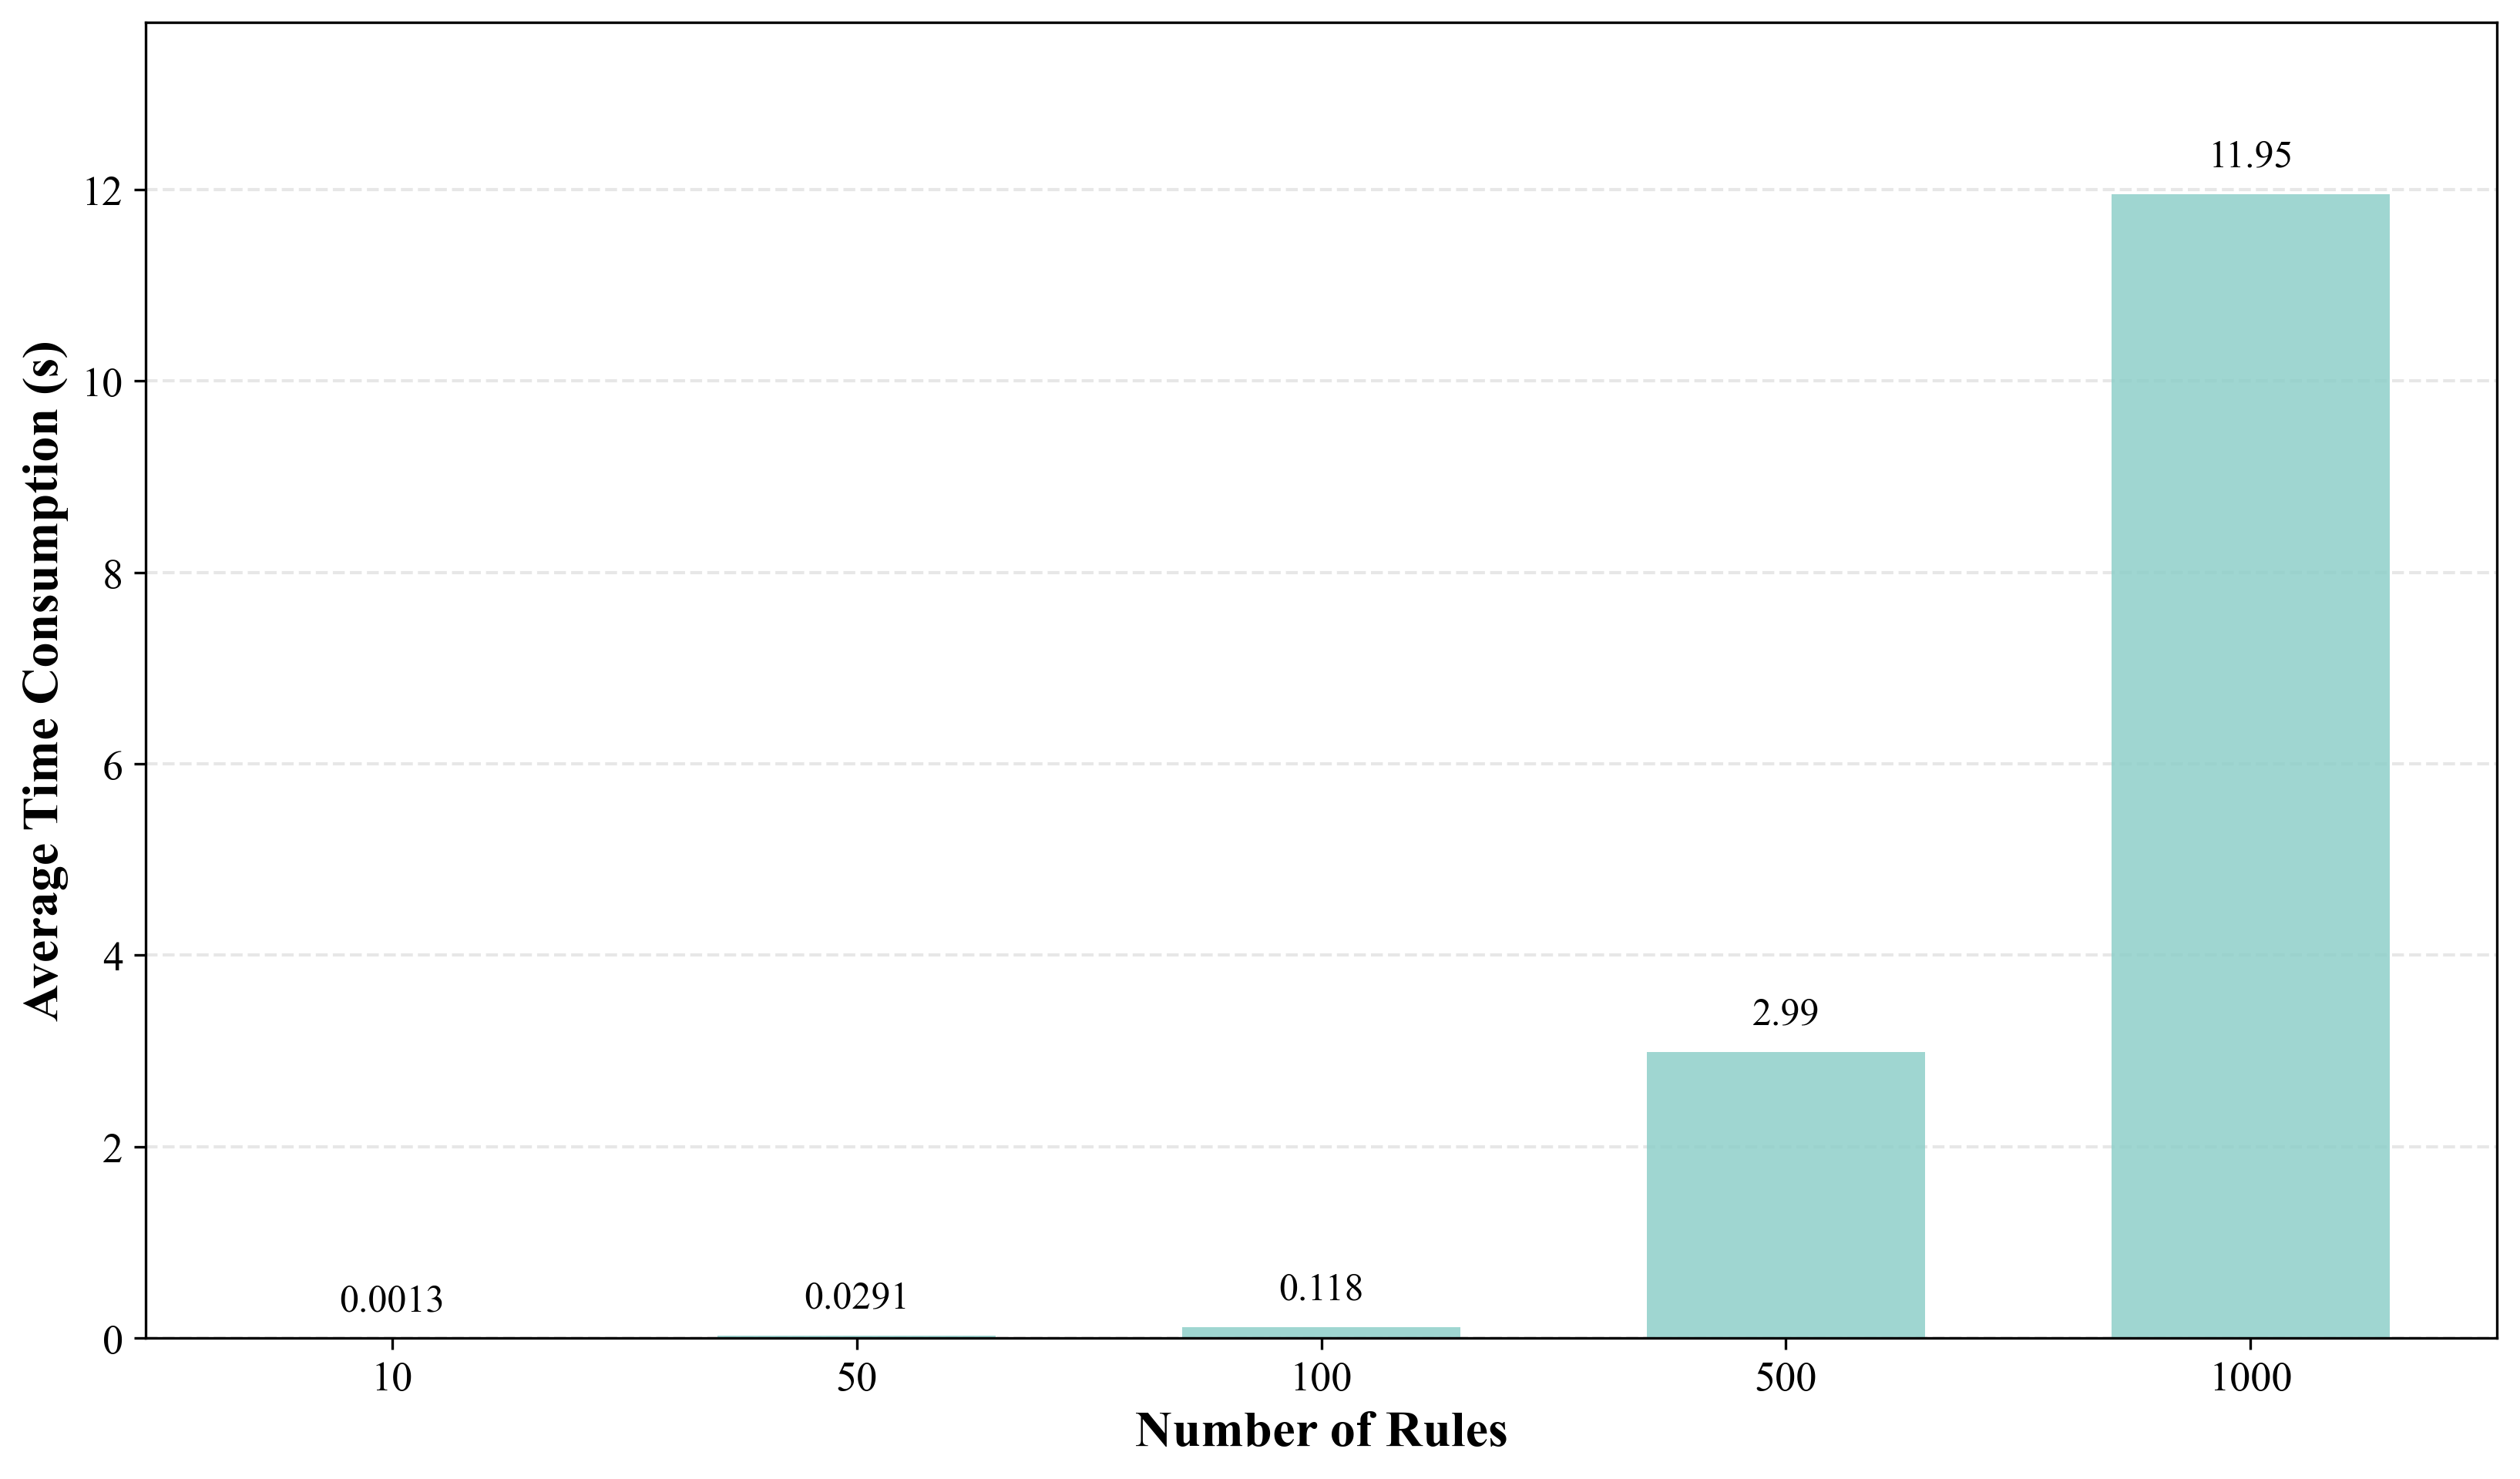
\includegraphics[width=0.8\textwidth]{figure/performance.png}
%   \caption{Static analysis execution time under different rule-set sizes.}
%   \label{performance_static_analysis}
% \end{figure}

\begin{figure*}[t]
  \centering
  \begin{minipage}[t]{0.48\linewidth}
        \begin{subfigure}{\linewidth}
            \centering
            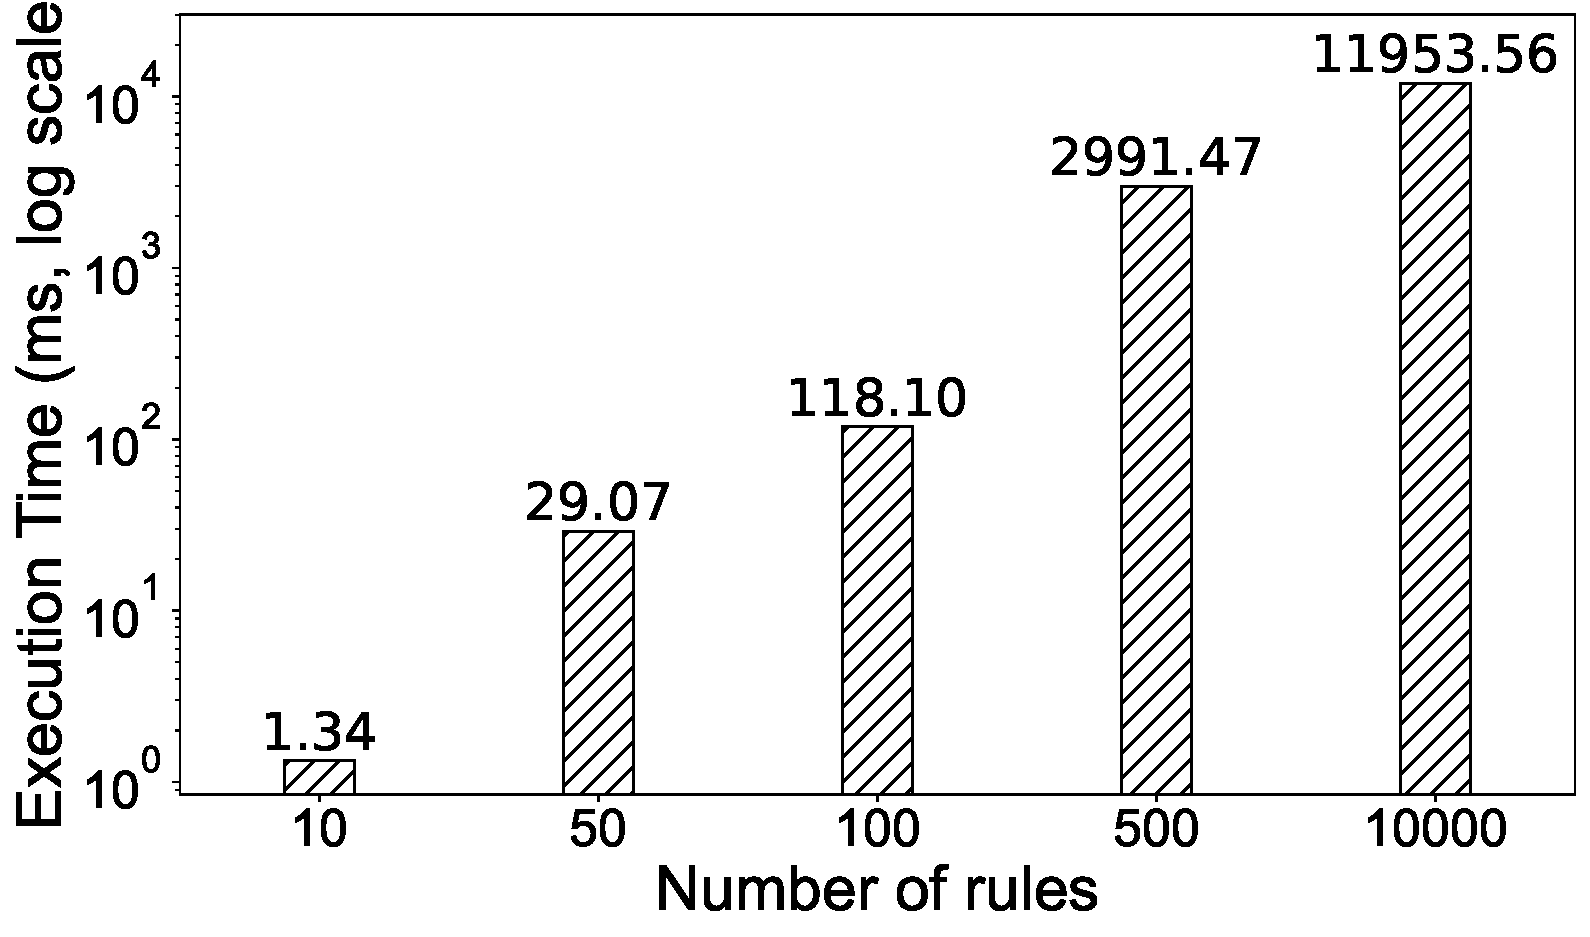
\includegraphics[width=\linewidth]{figure/static.pdf}
            \caption{Static analysis execution time under different rule-set sizes.}            
            \label{subfig:static}
        \end{subfigure}
  \end{minipage}
    \begin{minipage}[t]{0.48\linewidth}
        \begin{subfigure}{\linewidth}
            \centering
            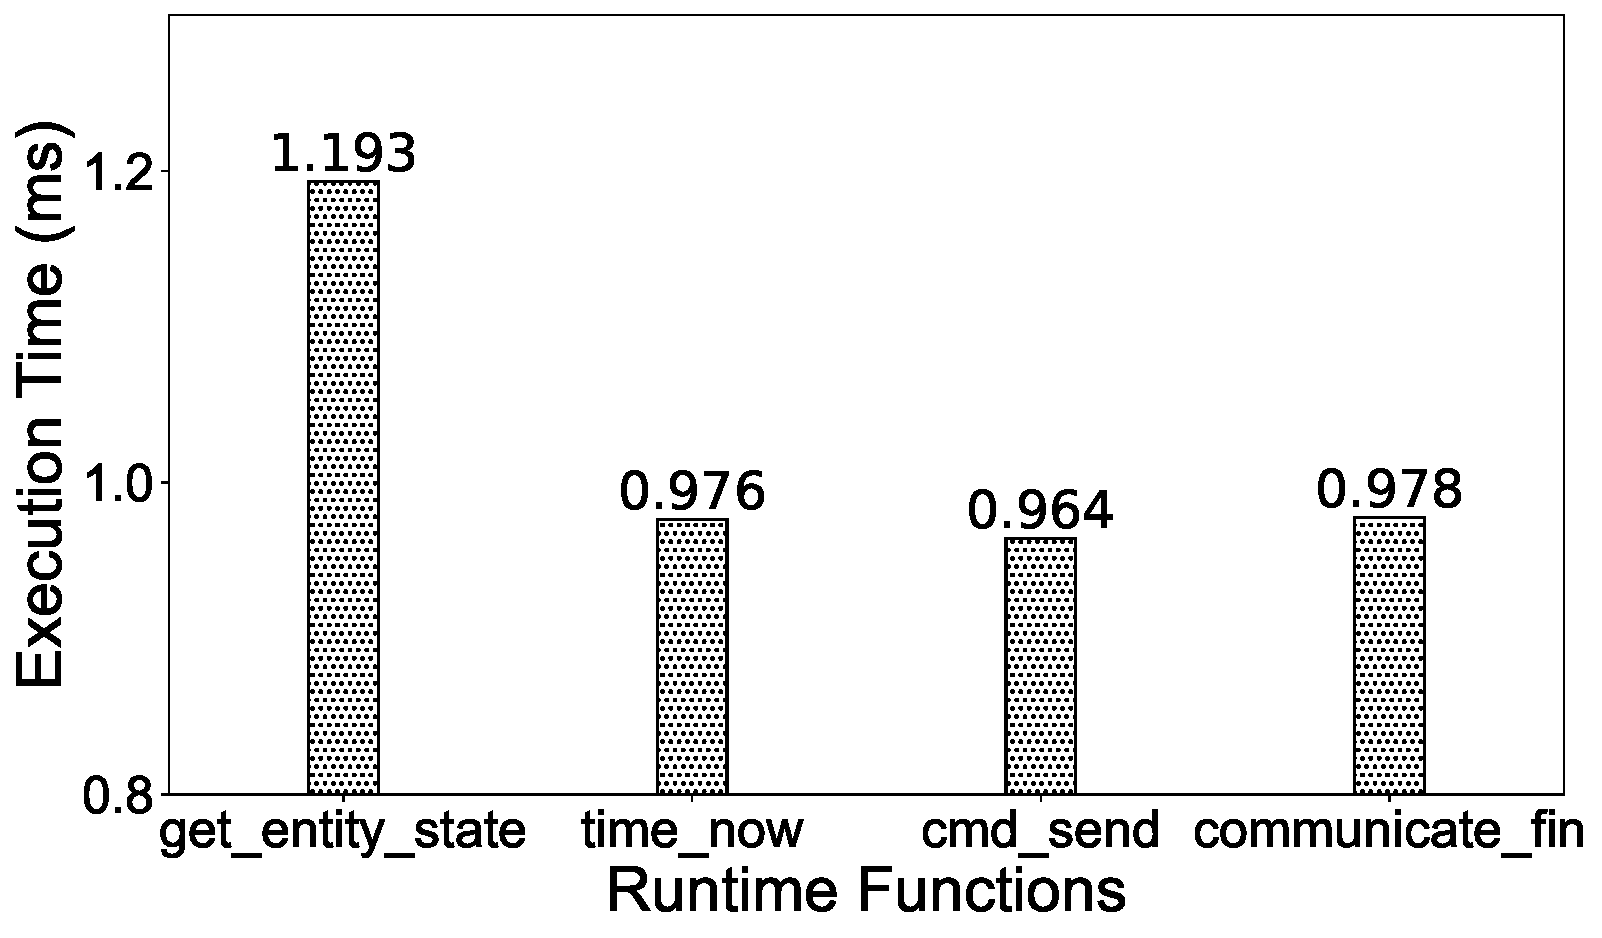
\includegraphics[width=\linewidth]{figure/runtime.pdf}
            \caption{Runtime verification execution time of different functions.}            
            \label{subfig:runtime}
        \end{subfigure}
  \end{minipage}
  \caption{The execution time of different components.}
  \label{fig:performance}
\end{figure*}

We evaluate the execution time of the static and runtime components of the framework.

\textbf{Static analysis.} The static phase constructs TCAE models, builds the RIDG, and extracts the RCDG. Figure~\ref{subfig:static} reports the average execution time on synthetically generated rule sets. Since the analysis checks pairwise interactions among automation rules, the time complexity is $O(n^2)$ for $n$ rules. Nevertheless, the overhead remains acceptable for offline use: the analysis finishes quickly for small and medium-sized rule sets and remains practical even for large rule sets. Because this phase is executed only after rule updates, it does not affect normal runtime operation.

\textbf{Runtime verification.} In the runtime phase, the main overhead comes from state retrieval and timestamp acquisition used by assertion verification. As shown in Fig.~\ref{fig:performance}(b), all runtime functions complete at the millisecond level. Among them, \texttt{get\_entity\_state} incurs the highest latency, while the other functions have similar and slightly lower overhead. Since each assertion verification requires only a small number of such calls, the overall runtime overhead remains low and is suitable for online dynamic monitoring.
\section{Related Work}

Prior work on rule conflict detection in smart home mainly falls into three lines: policy/property checking, physical-channel-aware analysis, and interaction-pattern-based hybrid detection. Huang et al.~\cite{huang2023survey} note that the problem definition, detection target, and conflict taxonomy are still not fully unified. We compare representative studies by whether they distinguish rule interaction from candidate rule conflicts (DIC) and whether they support user-specific safety preferences with reasonable user effort.

\textbf{Policy/property checking.} Soteria~\cite{celik2018soteria}, IoTGuard~\cite{celik2019iotguard}, SafeChain~\cite{hsu2019safechain}, and IoTSan~\cite{nguyen2018iotsan} verify predefined safety or security properties over IoT apps or trigger--action programs. These approaches are effective for checking explicit properties, but they rely heavily on expert-crafted policies or templates, which are difficult to generalize across diverse smart home deployments and often require substantial manual effort.

\textbf{Physical-channel-aware analysis.} iRuler~\cite{wang2019charting}, IoTIE~\cite{chen2019multi}, IoTSafe~\cite{ding2021iotsafe}, and IoTCom~\cite{alhanahnah2022iotcom} analyze interactions through physical channels to expose hidden dependencies beyond shared devices. However, their support for zone-dependent propagation is limited, absent, or dependent on deployment-specific input, which may over-approximate cross-zone effects and introduce false positives. IoTSafe further uses dynamic monitoring, but at the cost of substantial deployment and testing effort.

\textbf{Interaction-pattern-based hybrid detection.} Pattern-based systems summarize representative rule interaction patterns and flag automation rules that match them~\cite{trimananda2020understanding,chi2020cross,chi2023detecting}. These methods are useful for discovering suspicious rule interaction, but deciding whether a matched pattern should be treated as a candidate rule conflict still requires deployment-specific context. IoTMediator~\cite{chi2023detecting} combines static pre-screening with runtime dynamic monitoring and supports customized handling, yet its pattern-driven target is not directly aligned with DIC under user-specific safety preferences, which can lead to false positives.

Compared with these approaches, our framework uses the Entity Safety Configuration as a lightweight preference baseline to filter rule interaction into candidate rule conflicts, and then applies runtime assertion verification to confirm whether a candidate conflict edge is activated under the current system state. This design eliminates nine false positives reported by IoTMediator in our testbed while keeping the runtime overhead at the millisecond level.
\section{Conclusion}

This paper presents a hybrid framework for rule conflict detection in smart home by combining offline static analysis with runtime dynamic monitoring. The framework incorporates physical-channel information and the Entity Safety Configuration to identify candidate rule conflicts, and then uses runtime assertion verification to confirm whether a candidate conflict edge is activated under the current system state.

Evaluation on a Home Assistant prototype shows that the framework detects the manually confirmed conflict cases in the testbed, including cases involving physical channels and zone-dependent effects, while avoiding several non-conflict cases reported by IoTMediator. The results also show that static analysis can be performed offline and that the runtime overhead remains at the millisecond level.

\bibliographystyle{splncs04}
\bibliography{paper}

\end{document}